\documentclass[a4paper,12pt]{article}
\usepackage [utf8]{inputenc}
\usepackage [italian]{babel}
\usepackage{graphicx}
%\usepackage{grffile}
\usepackage{listings}
\usepackage{color}
\usepackage[hidelinks]{hyperref}
\usepackage{calc}
\usepackage{caption}

\addtolength{\oddsidemargin}{-40pt}
\addtolength{\textwidth}{80pt}
\addtolength{\voffset}{-60pt}
\addtolength{\textheight}{100pt}


\graphicspath{ {../Schema concettuale} {../Schema logico relazionale} {../Piani di accesso} }
\lstset{inputpath=../Sorgenti SQL/}

\definecolor{codegreen}{rgb}{0,0.6,0}
\definecolor{codegray}{rgb}{0.5,0.5,0.5}
\definecolor{codepurple}{rgb}{0.58,0,0.82}
\definecolor{backcolour}{rgb}{0.95,0.95,0.92}

\lstdefinestyle{mystyle}{
    language=SQL,
    backgroundcolor=\color{backcolour},   
    commentstyle=\color{codegreen},
    keywordstyle=\color{magenta},
    numberstyle=\small\color{codegray},
%    xleftmargin=-10px,
    stringstyle=\color{codepurple},
    basicstyle=\ttfamily,
    breakatwhitespace=false,         
    breaklines=true,                 
%    captionpos=b,                    
    keepspaces=true,                 
    numbers=left,                    
    numbersep=10pt,                  
    showspaces=false,
    showstringspaces=false,
    showtabs=true,
    tabsize=4
}
\lstset{style=mystyle}

\addto\captionsitalian{%
\renewcommand{\lstlistingname}{Codice}}
\addto\captionsitalian{%
\renewcommand{\lstlistlistingname}{Elenco dei listati di codice}}


%%%%%%%%%%%%%%%%%%%%%%%  FRONTESPIZIO %%%%%%%%%%%%%%%%%%%%%%%

\title { \vspace{-1.0cm}{\small Università di Pisa\\Dipartimento di Informatica\\Corso di Laurea in Informatica\\[0.5cm]Corso di Basi di Dati (244AA), prof. Giorgio Ghelli\\[0.7cm]}Progetto ``Studio professionale fatture"\\Relazione finale }
\author { Candidati:\\Alessandro Antonelli\\(matricola 507264, corso A)\\Tony Agosta\\(matricola 544090, corso A)}
\date { Consegna: 25 marzo 2021\\Appello straordinario marzo 2021\\A.A. 2019/2020 }

\begin {document}
 \maketitle
 
 \tableofcontents

\listoffigures

\lstlistoflistings

 \clearpage
 
%%%%%%%%%%%%%%%%%%%%%%%  CONTENUTO %%%%%%%%%%%%%%%%%%%%%%%

 \section{ Descrizione del dominio }

Bla bla bla

 \section{ Schema concettuale }

\begin{minipage}{\textwidth}
\begin{center}
\centering 
 \captionof{figure}{Schema concettuale a oggetti}
\centerline{
%\frame{
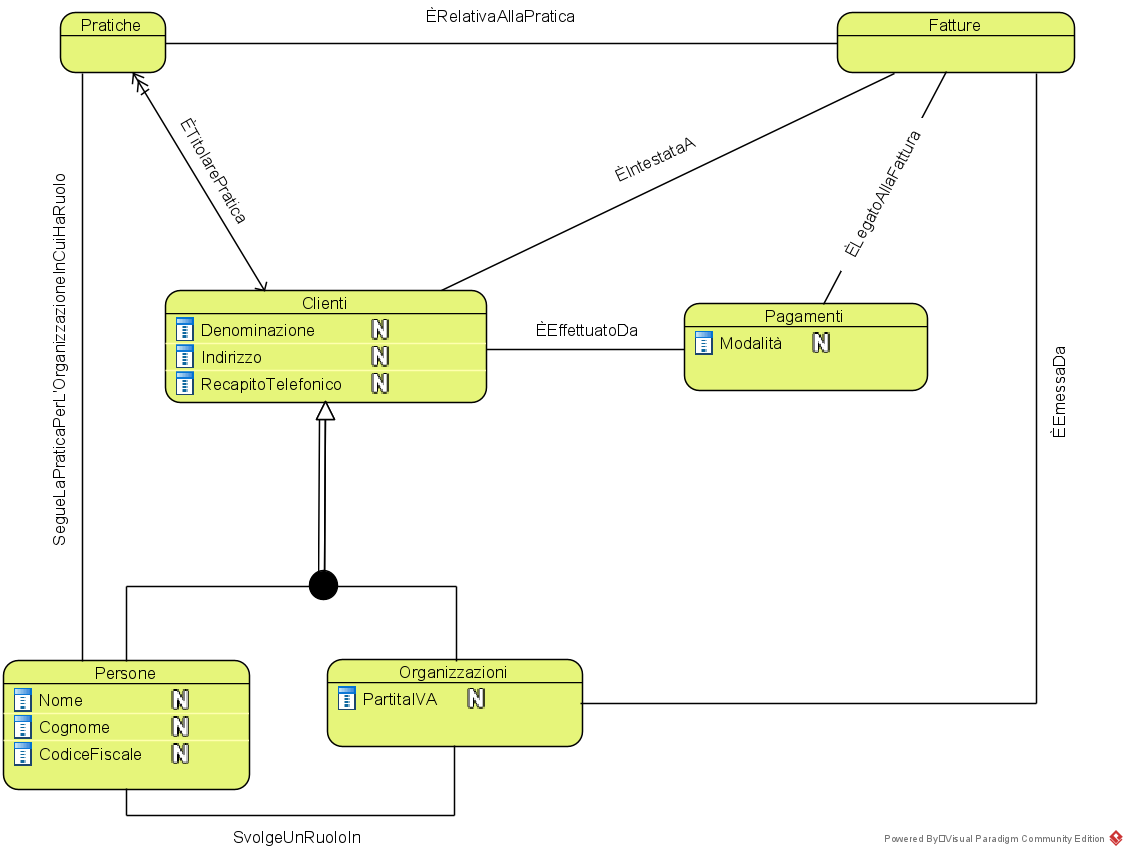
\includegraphics[width=\textwidth]{ Schema concettuale a oggetti.png }
}
\end{center}
\end{minipage}

 \subsection{ Vincoli }

\subsection{ Vincoli intrarelazionali }

\begin{itemize}
\item Tutti gli attributi (comprese le chiavi esterne) hanno il vincolo NOT NULL.

\item Il \textit{Nome} e il \textit{Cognome} di una \textit{Persona} deve essere lungo almeno 1 carattere.

\item Il \textit{CodiceFiscale} di una \textit{Persona} deve essere lungo esattamente 16 caratteri.

\item L'\textit{Importo} di una \textit{Fattura} deve essere $>$ 0.

\item La \textit{CifraPagata} di un \textit{Pagamento} deve essere $>$ 0.

\item La \textit{PartitaIVA} di un'\textit{Organizzazione} deve essere di esattamente 11 caratteri.

\item Il \textit{RecapitoTelefonico} di un \textit{Cliente} non può essere lungo meno di 9 caratteri.

\item La \textit{Qualifica} di un \textit{RuoloAziendale} deve essere presente ... ?
\end{itemize}

\subsection{ Vincoli interrelazionali }

\begin{itemize}
\item La \textit{CifraPagata} di un \textit{Pagamento} deve essere $\leq$ dell'\textit{Importo} della \textit{Fattura} a cui si riferisce.

\item Se il titolare di una \textit{Pratica} è un cliente che è una \textit{Organizzazione}, allora la \textit{Pratica} deve essere seguita da almeno un \textit{RuoloAziendale}.
\end{itemize}

 \section{ Schema logico relazionale }

 \subsection{ Formato grafico }

\begin{minipage}{\textwidth}
\begin{center}
\centering 
 \captionof{figure}{Schema logico relazionale}
\centerline{
%\frame{
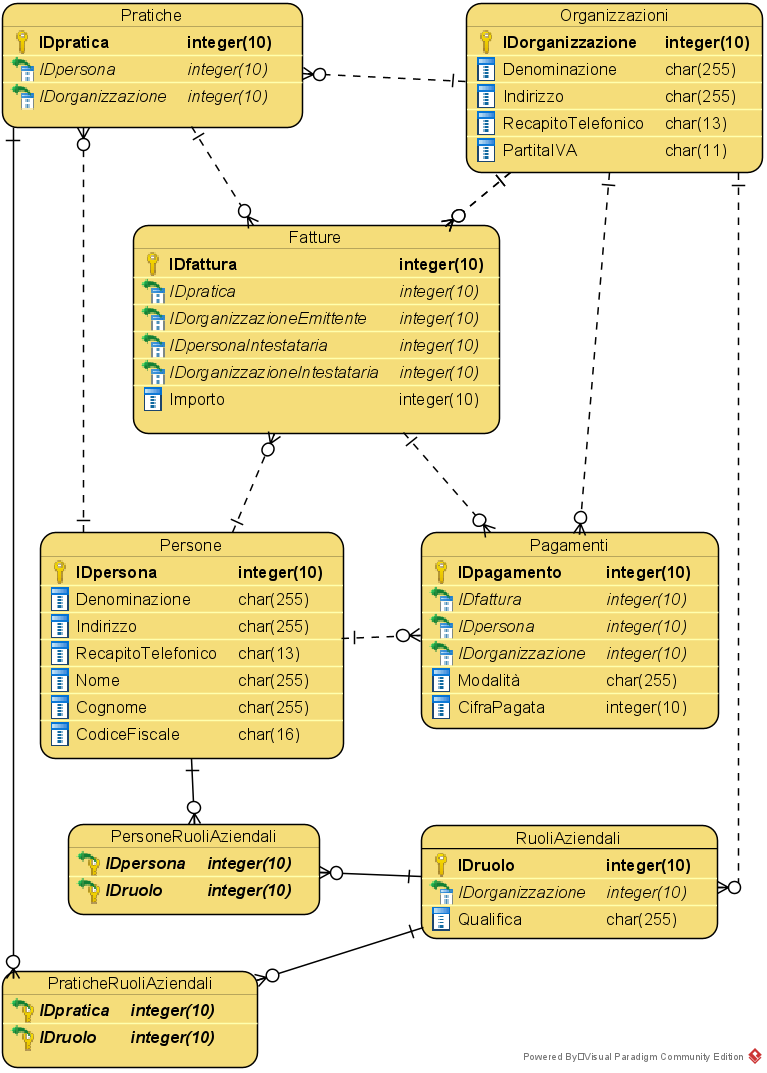
\includegraphics[width=\textwidth -4cm]{ Schema logico relazionale.png }
}
\end{center}
\end{minipage}

 \subsection{ Formato testuale }

\begin{itemize}
\item \textbf{Pratiche} (\underline{IDpratica}, IDpersona*, IDorganizzazione*)

\item \textbf{Fatture} (\underline{IDfattura}, IDpratica*, IDorganizzazioneEmittente*, IDpersonaIntestataria*, IDorganizzazioneIntestataria*, Importo)

\item \textbf{Persone} (\underline{IDpersona}, Denominazione, Indirizzo, RecapitoTelefonico, Nome, Cognome, CodiceFiscale)

\item \textbf{Organizzazioni} (\underline{IDorganizzazione}, Denominazione, Indirizzo, RecapitoTelefonico, PartitaIVA)

\item \textbf{Pagamenti} (\underline{IDpagamento}, IDfattura*, IDpersona*, IDorganizzazione*, Modalità, CifraPagata)

\item \textbf{PersoneRuoliAziendali} (\underline{IDpersona*}, \underline{IDruolo*})

\item \textbf{PraticheRuoliAziendali} (\underline{IDpratica*}, \underline{IDruolo*})

\item \textbf{RuoliAziendali} (\underline{IDruolo}, IDorganizzazione*, Qualifica)
\end{itemize}


 \subsection{ Dipendenze funzionali }

 \subsubsection{ Relazioni A, B, C }

 \subsubsection{ Relazioni C, D, E }

 \subsubsection{ Relazioni X }

 \section{ Interrogazioni }

 \subsection{ Uso di proiezione, join e restrizione }
 \subsection{ Uso di group by con having, where e sort }
 \subsection{ Uso di join, group by con having e where }
 \subsection{ Uso di select annidata con quantificazione esistenziale }
 \subsection{ Uso di select annidata con quantificazione universale }
 \subsection{ Uso di subquery di confronto quantificato usando una subquery }

\lstinputlisting[caption=esempio]{esempio.sql}

 \section{ Piani di accesso }

 \subsection{ Piani di accesso logico }

 \subsubsection{ Query 1) }

 \subsubsection{ Query 2) }

 \subsubsection{ Query 3) }

 \subsection{ Piani di accesso fisico senza uso di indici }

 \subsubsection{ Query 1) }

 \subsubsection{ Query 2) }

 \subsubsection{ Query 3) }

 \subsection{ Piani di accesso fisico con uso di indici }

 \subsubsection{ Query 1) }

 \subsubsection{ Query 2) }

 \subsubsection{ Query 3) }

\end{document}